\section{Case studies}
For conducting experiments two setups were used. A basic one consisted only from one DC motor. The second was \textsf{The Velvet Fingers}.

\subsection{Basic methods}
Three fundamental methods of control are: current, position and velocity control. They all rely on measuring one process variable (PV) and try to reach the setpoint (SP) with use of a PID controller, which output is the control variable (CV).

\begin{equation}
u(t) = K_p e(t) + K_i \int_{0}^{t}e(\tau)d\tau + K_d \frac{de}{dt} 
\end{equation}

\subsubsection{Current Control}
Current control can be identified with force control. Even though there are no tactile sensors, hence the force is not explicitly measured, the  applied force can be implicitly calculated from \ref{eq:curr_force}. 

\begin{figure}%[H]
 \begin{center} 
  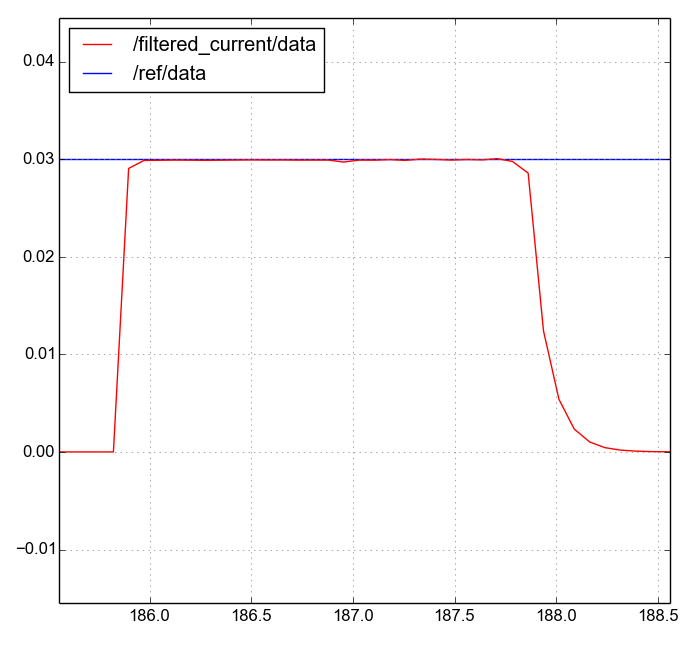
\includegraphics[width=0.55\textwidth]{./stuff/filtered_current}
 \end{center}
 \caption{An exaple plot of the current control}
 \label{fig:current_plot} 
\end{figure}   

Figure \ref{fig:current_plot} presents changes of current flowing through the motor in time. X-axis is time [s], Y-axis is current [A]. We can see three phases: in the beginning and the end the motor was running without any constraints, in the middle phase the movement was constrained.
The response was almost instantaneous, and the control variable reached the setpoint very precisely and without oscillations. 

\subsubsection{Position Control}
\begin{figure}%[H]
 \begin{center} 
  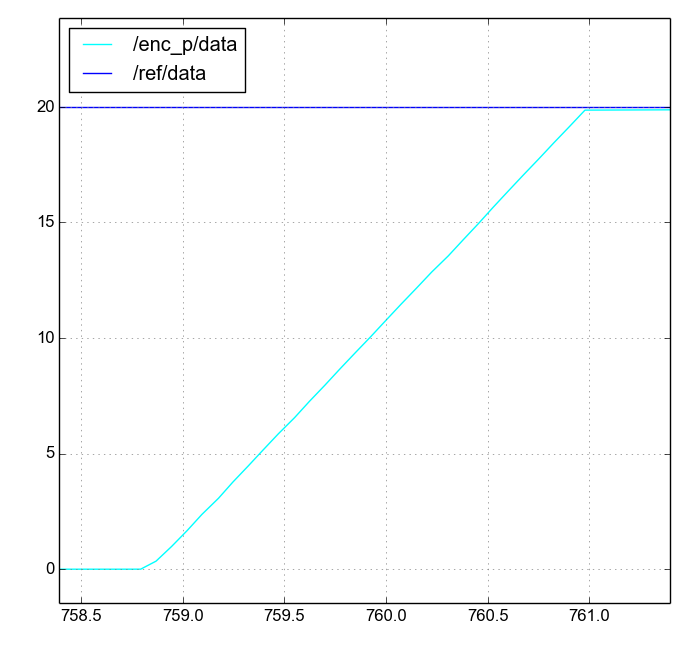
\includegraphics[width=0.55\textwidth]{./stuff/enc_p_plot}
 \end{center}
 \caption{An exaple plot of the position control}
 \label{fig:position_plot} 
\end{figure} 

Figure \ref{fig:position_plot} presents changes of the motor's position in time. X-axis is time [s], Y-axis is position [rad]. After applying the voltage the movement was steady.
The control variable reached the setpoint very precise and without oscillations.

\subsubsection{Velocity Control}
\begin{figure}%[H]
 \begin{center} 
  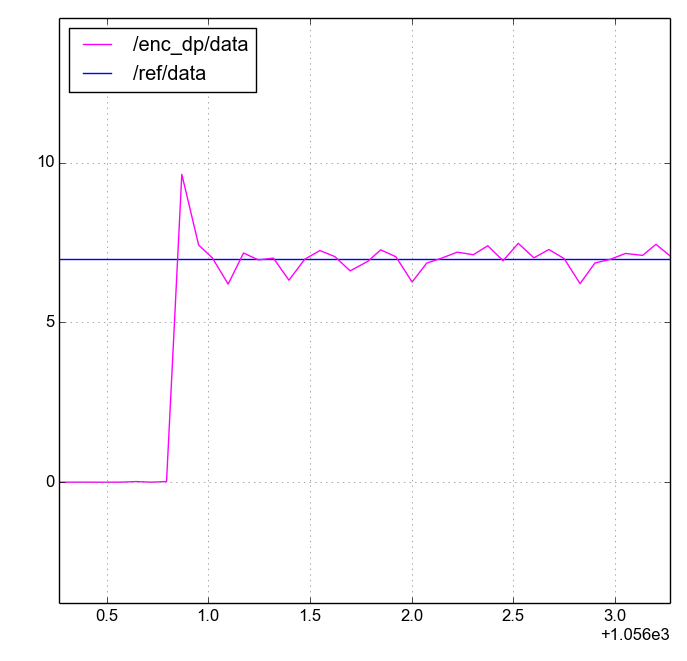
\includegraphics[width=0.55\textwidth]{./stuff/enc_dp_plot}
 \end{center}
 \caption{An exaple plot of the velocity control}
 \label{fig:velocity_plot} 
\end{figure} 

Figure \ref{fig:velocity_plot} presents changes of the motor's velocity in time. X-axis is time [s], Y-axis is angular velocity [rad/s]. After applying the voltage the motor reached the setpoint very fast. Although oscillations are presented in the plot, the movement of the motor was actually smooth. The oscillations are visible due to measurements done by encoder and derivating the position, which introduce some noise.

\subsection{Complex methods}
When interacting with the environment, there is need for more sophisticated methods. The control variable is calculated based on two or more process variables.

Nomenclature: $p$ - current position, $\dot{p}$ - current velocity, $\ddot{p}$ - current acceleration, $f$ - current force, $_d$ - desired value, $K_p$ - position coefficient, $K_v$ - velocity coefficient, $K_f$ - force coefficient, $K_i$ - integral coefficient, $M$ - mass, $B$ - damping, $K$ - stiffness.

\subsubsection{Stiffness Control}
Stiffness control derives from a position control scheme of PD type.

\begin{equation}
u(t) = K_{p}(p_{d} - p) - K_{v} \dot{p},
\end{equation}

\begin{figure}%[H]
 \begin{center} 
  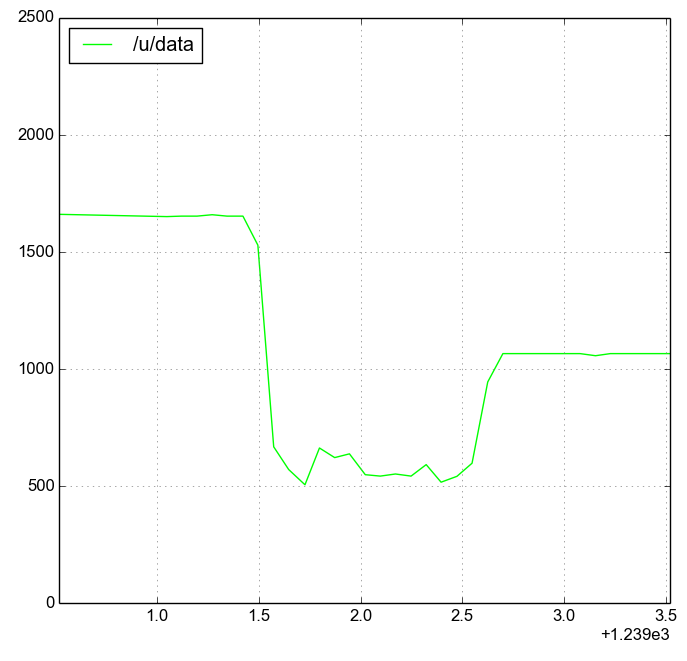
\includegraphics[width=0.55\textwidth]{./stuff/stiffness_plot}
 \end{center}
 \caption{An exaple plot of the stiffness control}
 \label{fig:stiffness_plot} 
\end{figure} 

Figure \ref{fig:stiffness_plot} presents changes of the control variable in time. X-axis is time [s], Y-axis is the CV. We can see three phases: in the beginning and the end the movement is constrained, in the middle phase the motor is running without any constraints.
When in contact with the environment, the CV is steady and larger than during the unconstrained motion.
Since stiffness control derives from a position control, the closer to the setpoint, the lower the CV. 

\subsubsection{Impedance Control}
In impedance control the input is flow (velocity or displacement) and the output is effort (force).
In directions where the robot has to be environment-sensitive, impedance is low, otherwise impedance is high. The desired impedance behavior is a trade-off between trajectory error and force error. If the motion is unconstrained, force will be zero and the robot will move to the reference position. 

\begin{equation}
u(t) = M(\ddot{p}_d - \ddot{p}) + B(\dot{p}_d-\dot{p}) + K(p_d-p) - K_f f
\end{equation}

Desired acceleration and velocity are usually not present to guarantee passivity when in contact with the environment.

\begin{figure}%[H]
 \begin{center} 
  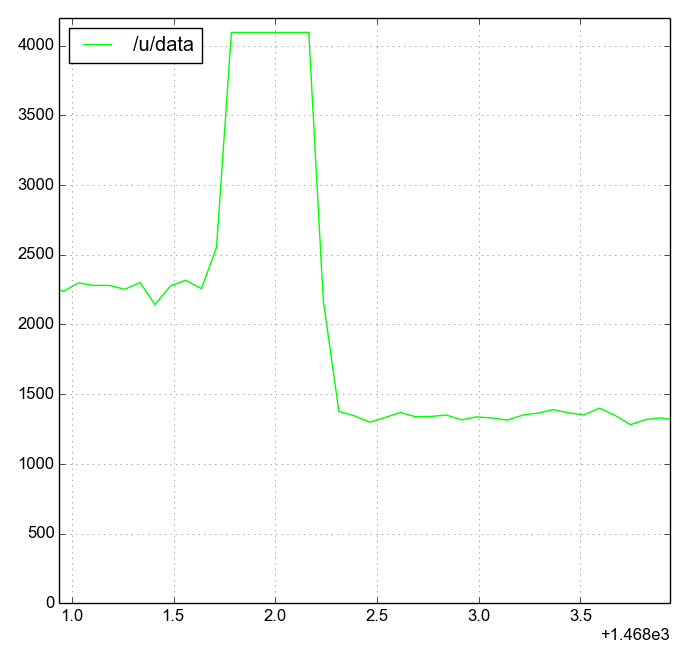
\includegraphics[width=0.55\textwidth]{./stuff/impedance_plot}
 \end{center}
 \caption{An exaple plot of the impedance control}
 \label{fig:impedance_plot} 
\end{figure} 

Figure \ref{fig:impedance_plot} presents changes of the control variable in time. X-axis is time [s], Y-axis is the CV. We can see three phases: in the beginning and the end the movement is constrained, in the middle phase the motor is running without any constraints.
When in contact with the environment, the CV is steady and smaller than during the unconstrained motion.
Such behaviour keeps the interaction force in desired boundaries and guarantees reaching the setpoint, if possible.
 
\subsubsection{Parallel Force/Position Control}
In order to combine features of stiffness control and force control, a parallel force/position regulator can be designed where a PI force control action plus desired force feedforward is used in parallel to a PD position control action.
The position controller is an impedance while the force controller results in a filtering action on the force variables.
 
\begin{equation}
u(t) = M \ddot{e}_p +  K_{v} \dot{e}_p + K_p e_p + K_f e_f + K_i\int_{0}^{t} e_f d\tau,
\end{equation}
where error $e$
\begin{equation}
e_{variable}(t) = variable_{desired} - variable(t).
\end{equation}

\begin{figure}%[H]
 \begin{center} 
  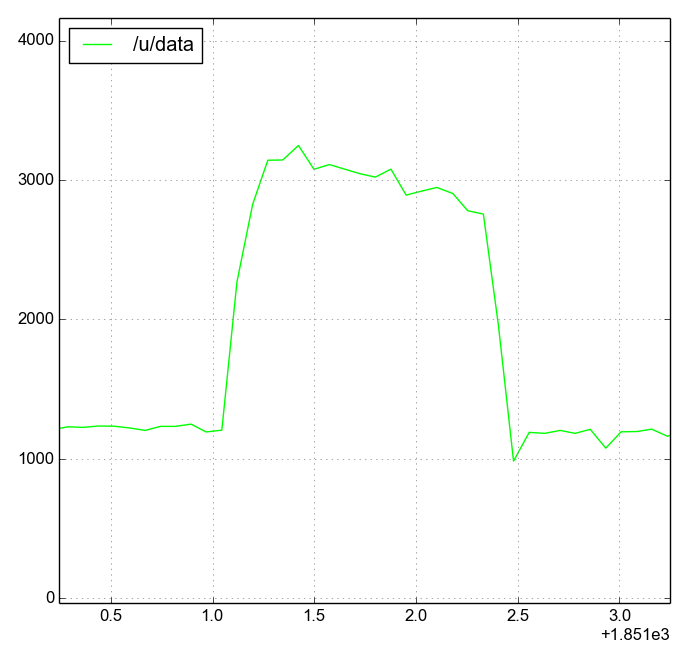
\includegraphics[width=0.55\textwidth]{./stuff/force_pos_plot}
 \end{center}
 \caption{An exaple plot of the parallel force/position control}
 \label{fig:force_pos_plot} 
\end{figure} 

Figure \ref{fig:force_pos_plot} presents changes of the control variable in time. X-axis is time [s], Y-axis is the CV. We can see three phases: in the beginning and the end the movement is constrained, in the middle phase the motor is running without any constraints.
When in contact with the environment, the CV is steady and smaller than during the unconstrained motion. When moving freely and going in direction of the setpoint, the CV slowly decreases.
Such behaviour keeps the interaction force at desired level independently of the position error and guarantees reaching the setpoint, if possible.